\chapter{Технологическая часть}

\section{Выбор средств реализации}

В качестве языка программирования был выбран \textit{С++}~\cite{cpp}, так как в стандартной библиотеке языка присутствует поддержка всех структур данных, выбранных по результатам проектирования, а так же средствами языка можно реализовать все алгоритмы, выбранные в результате проектирования.

В качестве среды разработки была выбрана среда $Qt Creator$ вместе с $Qt$~\cite{qt}, так как у него есть встроенные функции для создания пользовательского интерфейса и встроенный отладчик.
Для тестирования был выбран фреймворк \textit{GoogleTest}~\cite{gtest}, так как я уже использовала его ранее и он предоставляет достаточный функционал для написания тестов для программы на \textit{С++}.

Для измерения времени будут использоваться функции \textit{$std::chrono::system\_clock::now(...)$} и \textit{$std::chrono::duration\_cast<std::chrono::milliseconds>$} из библиотеки $chrono$~\cite{cpp-lang-chrono}.

В качестве формата входного файла с фламинго был выбран формат $obj$~\cite{obj}, так как это распространенный формат для хранения 3D объектов и его обработка не требует большого количества  вычислительных действий или использования дополнительных библиотек.


\section{Графический интерфейс программы}

Пример пользовательского интерфейса представлен на рисунке (\ref{fig:inter}).
\clearpage
\begin{figure}[h!]
	\centering
	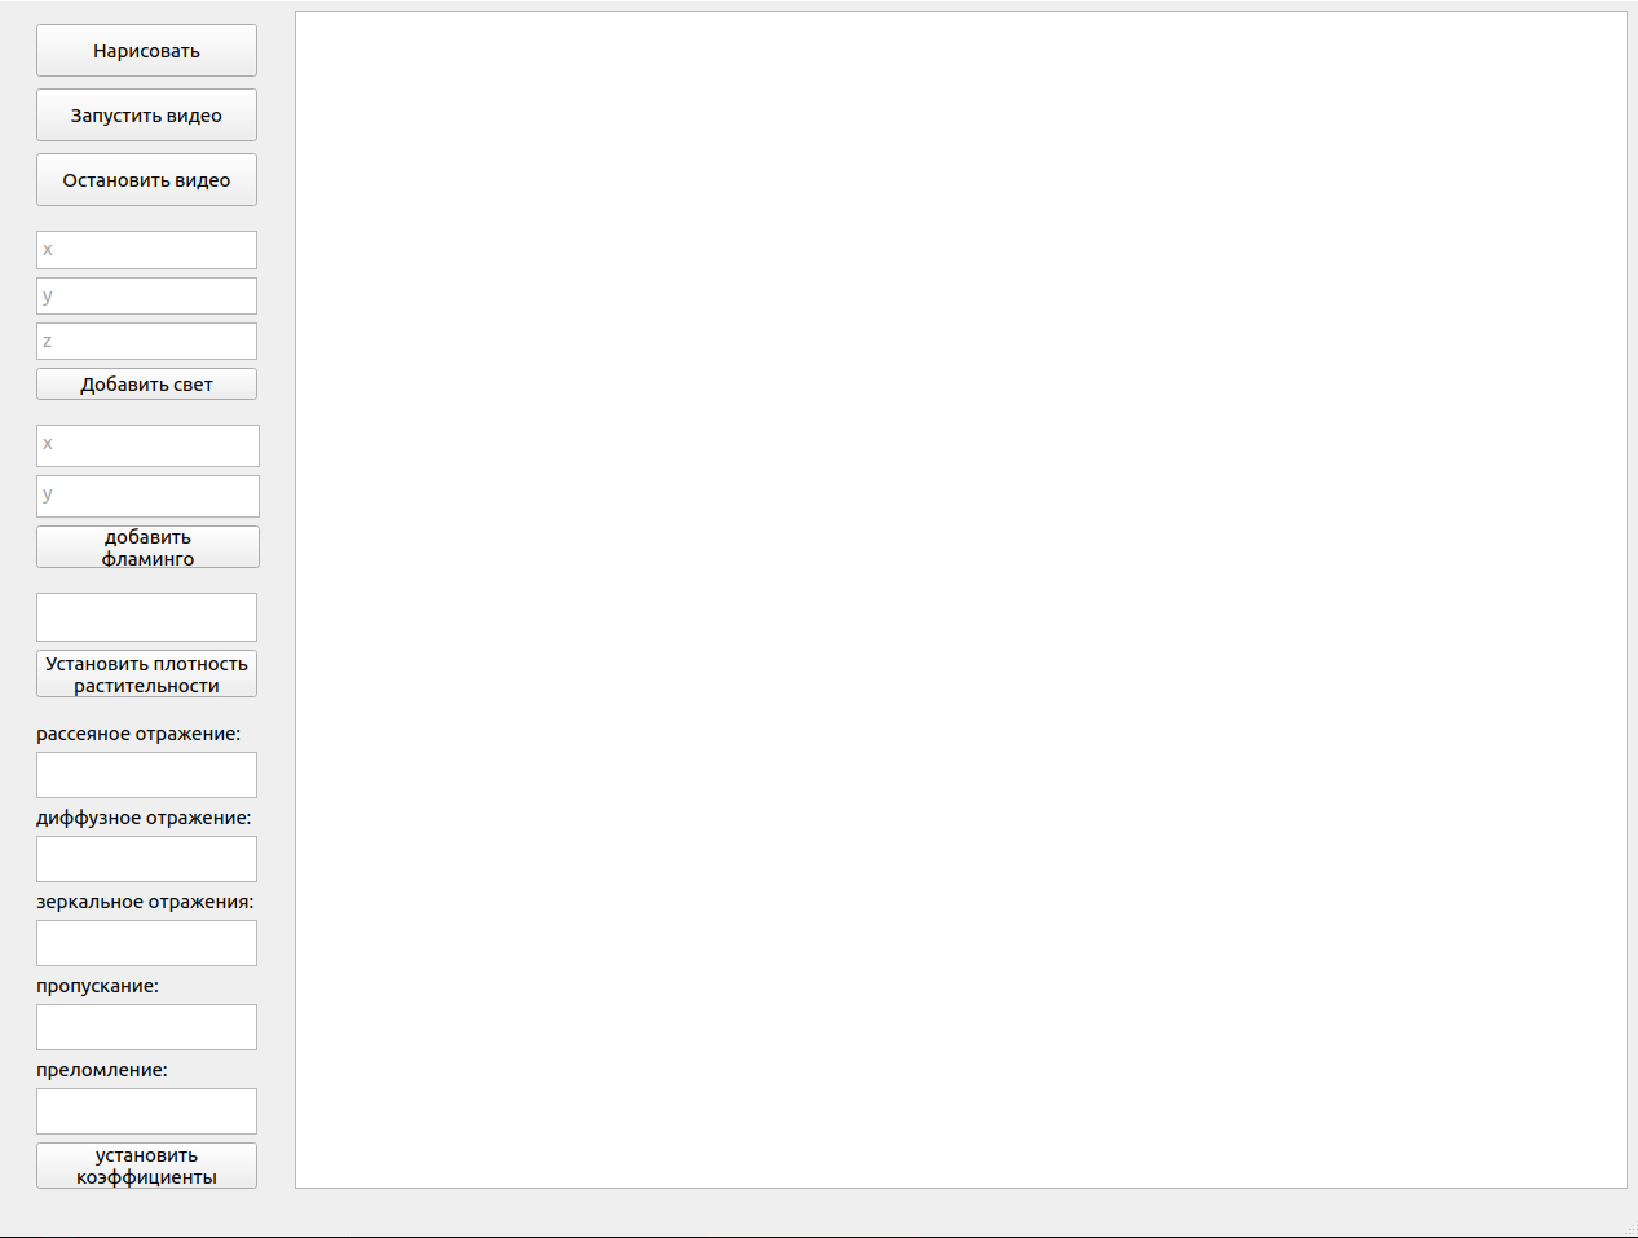
\includegraphics[width=0.9\linewidth]{img/inter}
	\caption{Пример интерфейса разработанной программы}
	\label{fig:inter}
\end{figure}

\section{Модульное тестирование}

Для модульного тестирования был использован фреймворк \textit{$Google Test$}.

Примеры модульных тестов, написанных для данной работы представлены в листингах~\ref{lst:mod_1}--\ref{lst:mod_3}.
\clearpage
\begin{center}
	\captionsetup{justification=raggedright,singlelinecheck=off}
	\begin{lstlisting}[label=lst:mod_1,caption={Тест для функции, которая определяет принадлежность точки полигону}]
TEST(IsInsideTest, IsInsideTest) {
	drawer dr;
	std::vector<QVector3D> points = {
		QVector3D(0, 0, 0),
		QVector3D(2, 1, 0),
		QVector3D(3, 5, 0)
	};
	int x = 1;
	int y = 2;
	bool result = dr.is_inside(x, y, points);
	EXPECT_TRUE(result);
}
	\end{lstlisting}
\end{center}


\begin{center}
	\captionsetup{justification=raggedright,singlelinecheck=off}
	\begin{lstlisting}[label=lst:mod_2,caption={Тест для функции, которая определяет прямоугольник, в который вписан полигон}]
TEST(DrawerTest, BorderTest2) {
	drawer dr = drawer(100, 100);
	std::vector<QVector3D> points = {
		QVector3D(-23, 0, 13),
		QVector3D(2, 102, 43),
		QVector3D(3, 5, 0),
		QVector3D(6, 4, 0)
	};
	std::tuple<int, int, int, int> result = dr.border(points);
	EXPECT_EQ(std::get<0>(result), 99); // ymax
	EXPECT_EQ(std::get<1>(result), 0); // ymin
	EXPECT_EQ(std::get<2>(result), 6); // xmax
	EXPECT_EQ(std::get<3>(result), 0); // xmin
}
	\end{lstlisting}
\end{center}
\clearpage

\begin{center}
	\captionsetup{justification=raggedright,singlelinecheck=off}
	\begin{lstlisting}[label=lst:mod_3,caption={Тест для функции, которая вычисляет коэффициенты плоскости}]
TEST(PlaneCoefTest, PlaneCoefTest) {
	drawer dr;
	std::vector<QVector3D> points = {
		QVector3D(4, 0, 0),
		QVector3D(67, 1, 9),
		QVector3D(2, 8, 3)
	};
	std::tuple<int, int, int, int> result = dr.plane_coef(points);
	EXPECT_EQ(std::get<0>(result), -69);   // a
	EXPECT_EQ(std::get<1>(result), -207); // b
	EXPECT_EQ(std::get<2>(result), 506);   // c
	EXPECT_EQ(std::get<3>(result), 276); // d
}
	\end{lstlisting}
\end{center}


\section{Примеры работы программы}

Примеры работы программы представлены на рисунках~(\ref{fig:ex1})--(\ref{fig:ex6}).

\begin{figure}[h!]
	\centering
	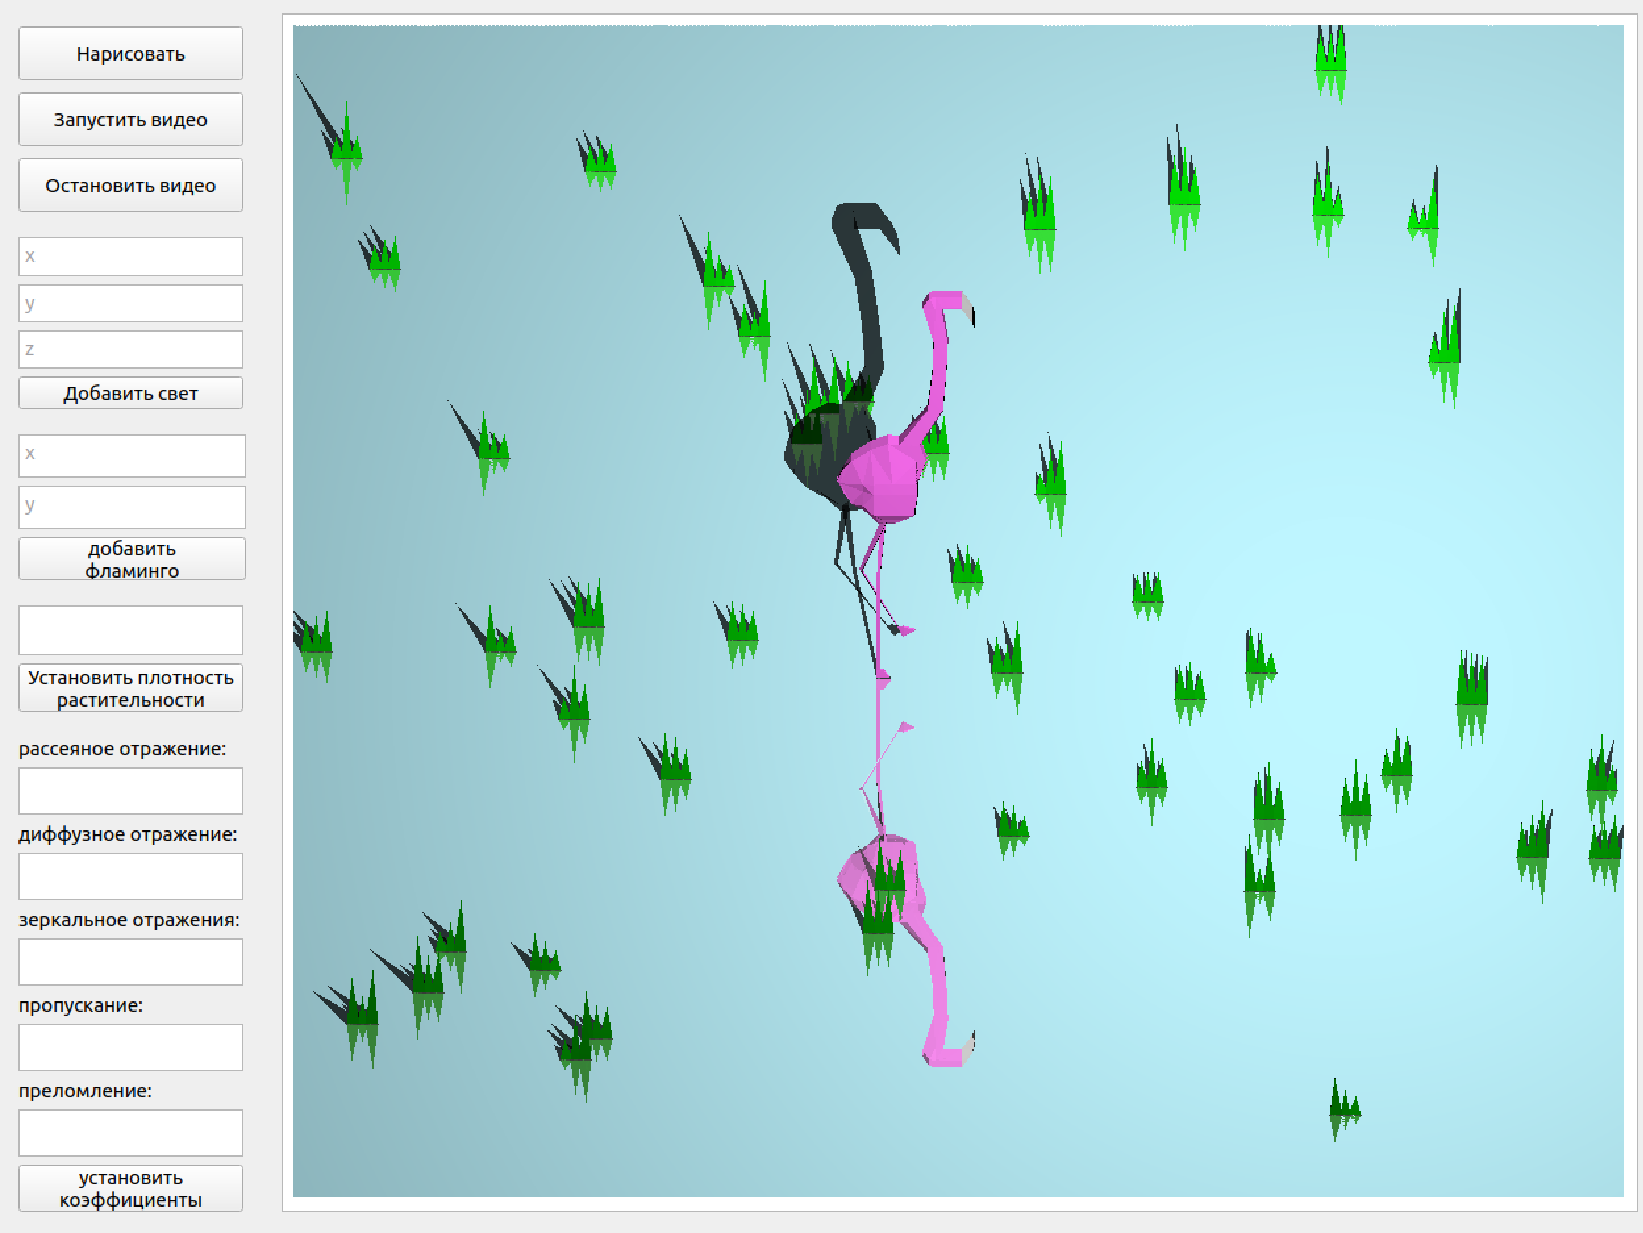
\includegraphics[width=0.8\linewidth]{img/ex1}
	\caption{Пример работы программы 1}
	\label{fig:ex1}
\end{figure}

\begin{figure}[h!]
	\centering
	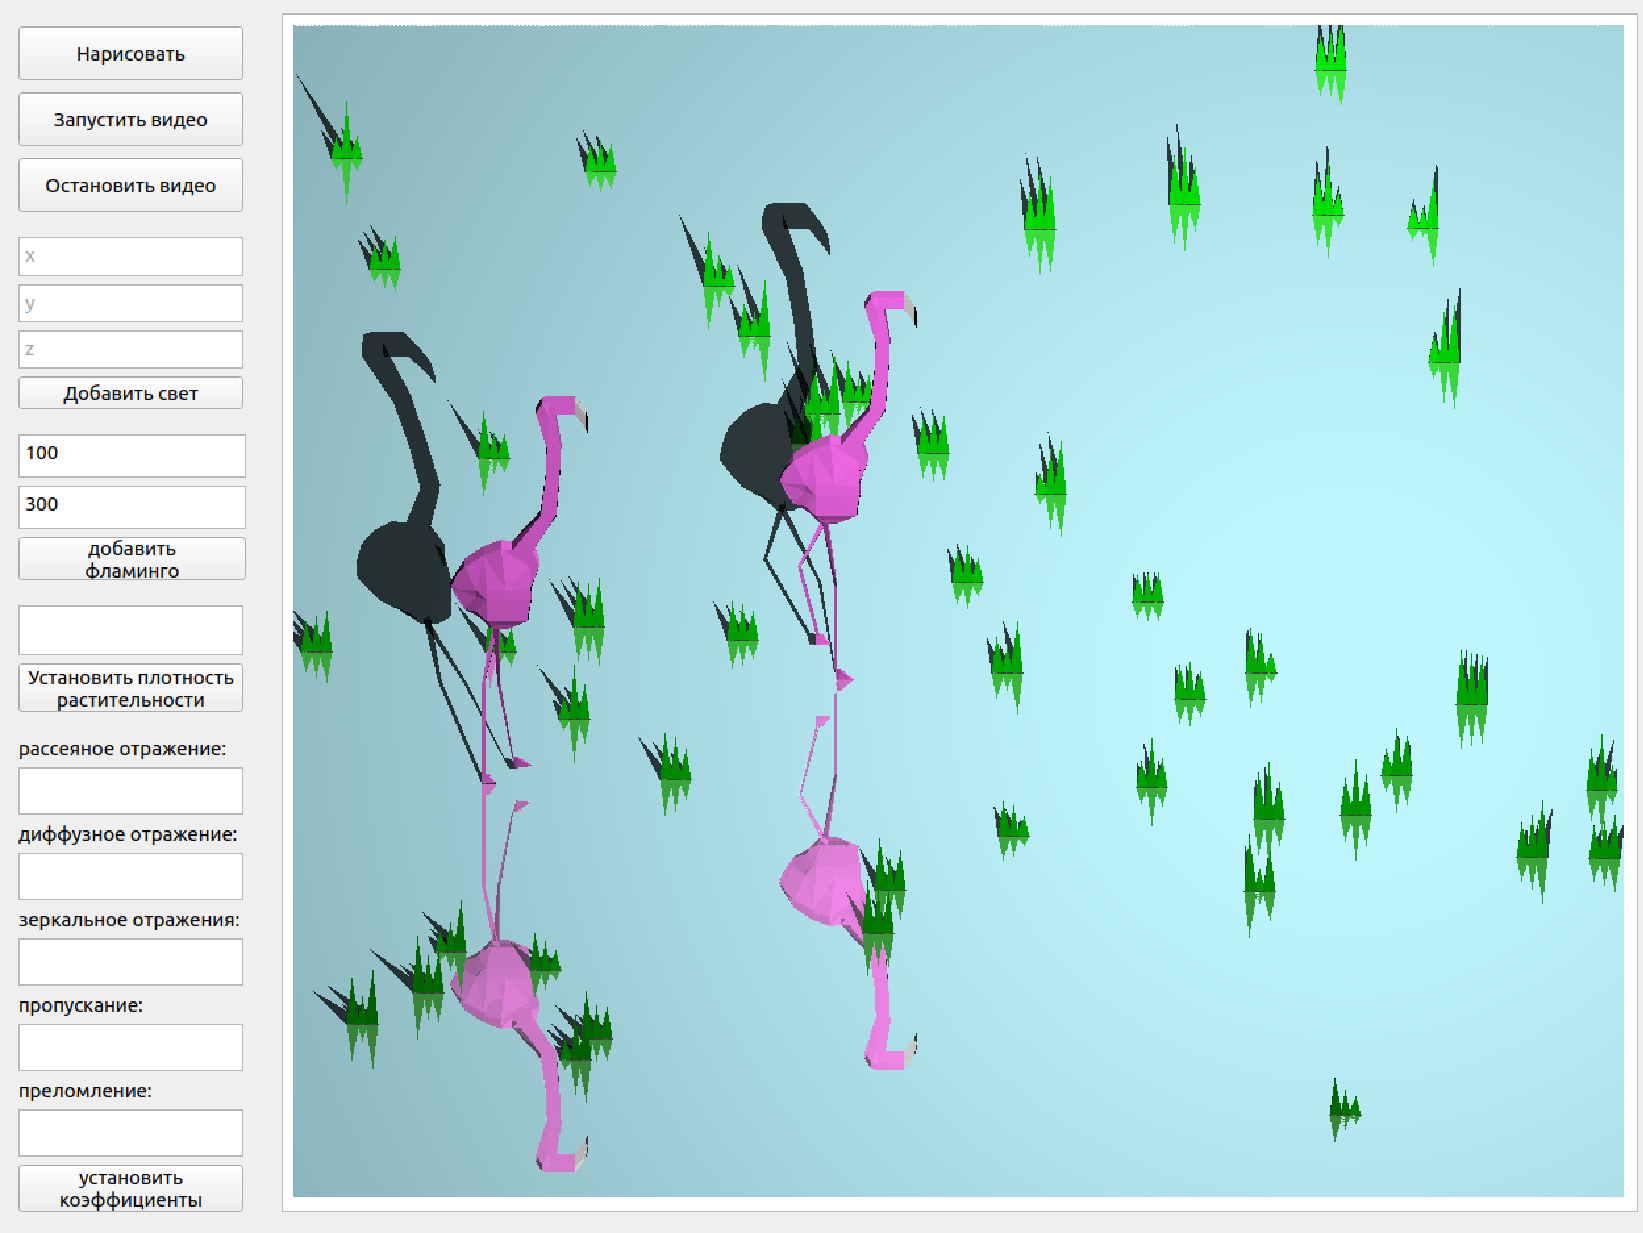
\includegraphics[width=0.9\linewidth]{img/ex2}
	\caption{Пример работы программы 2}
	\label{fig:ex2}
\end{figure}

\begin{figure}[h!]
	\centering
	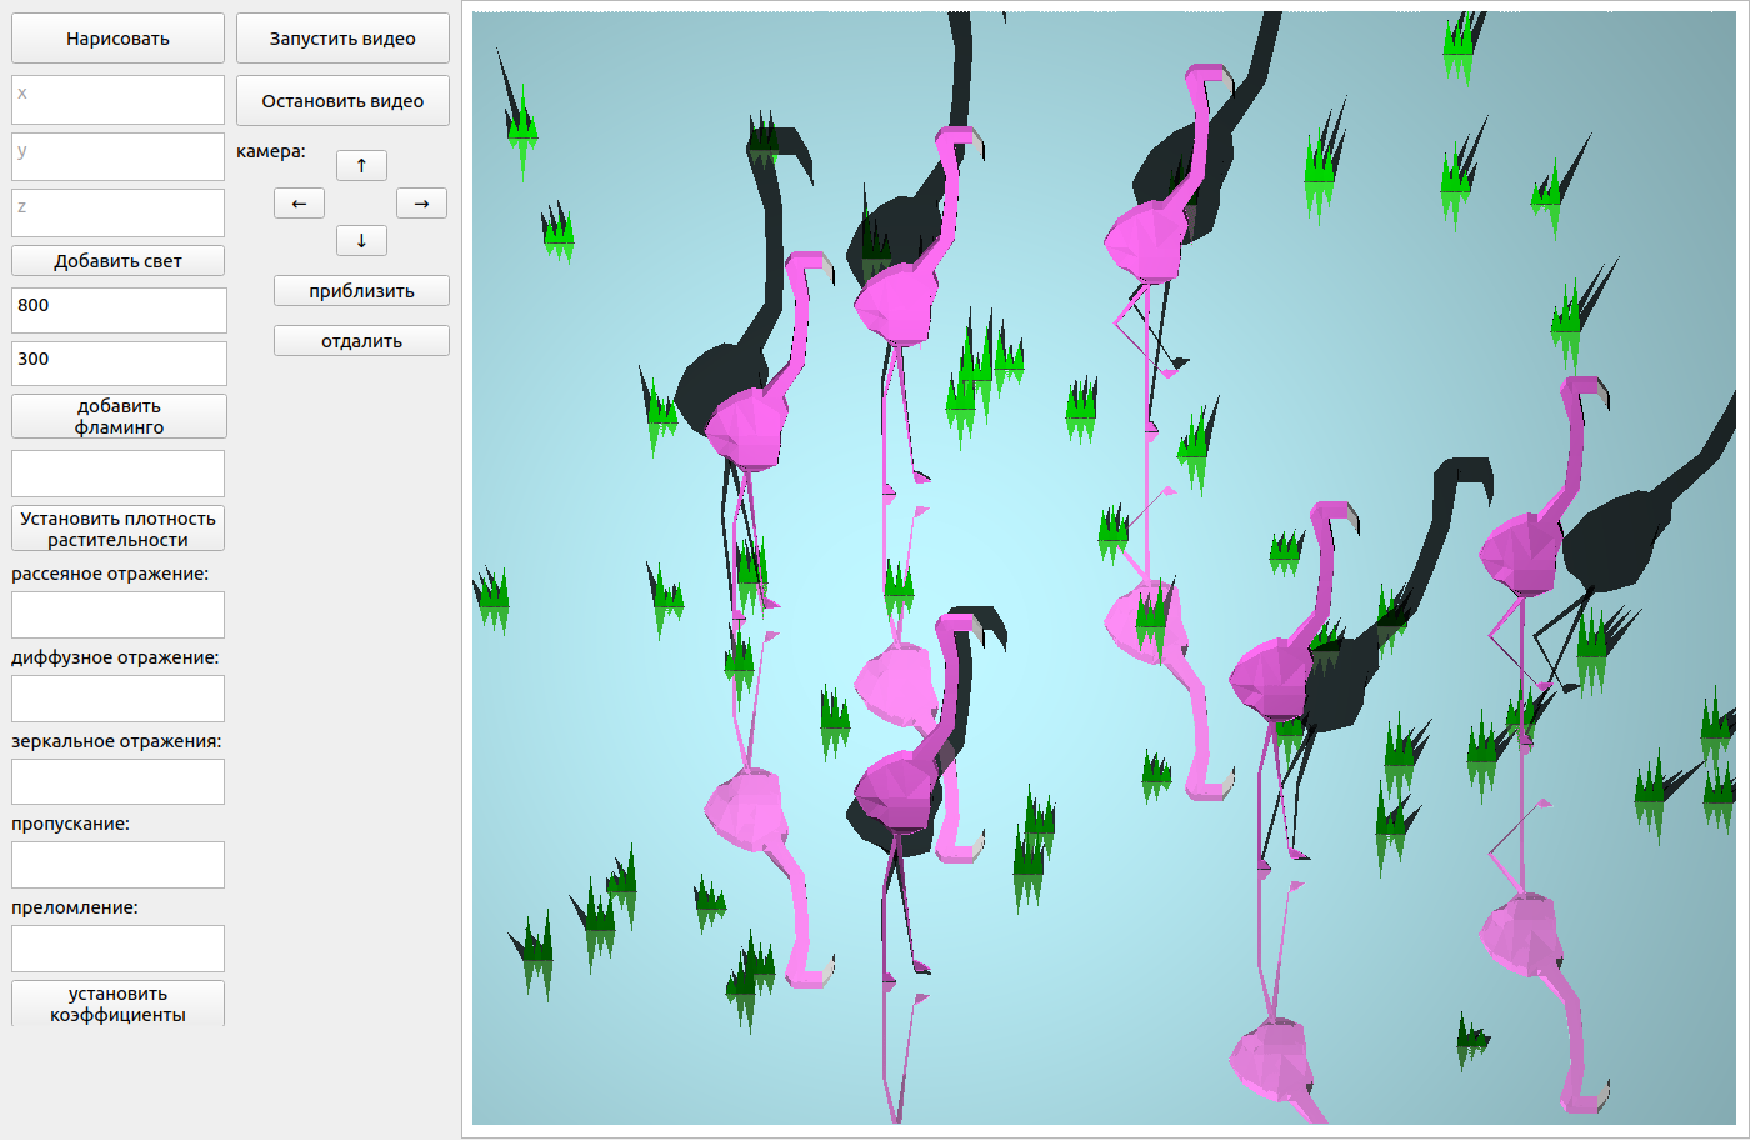
\includegraphics[width=0.9\linewidth]{img/ex3}
	\caption{Пример работы программы 3}
	\label{fig:ex3}
\end{figure}

\begin{figure}[h!]
	\centering
	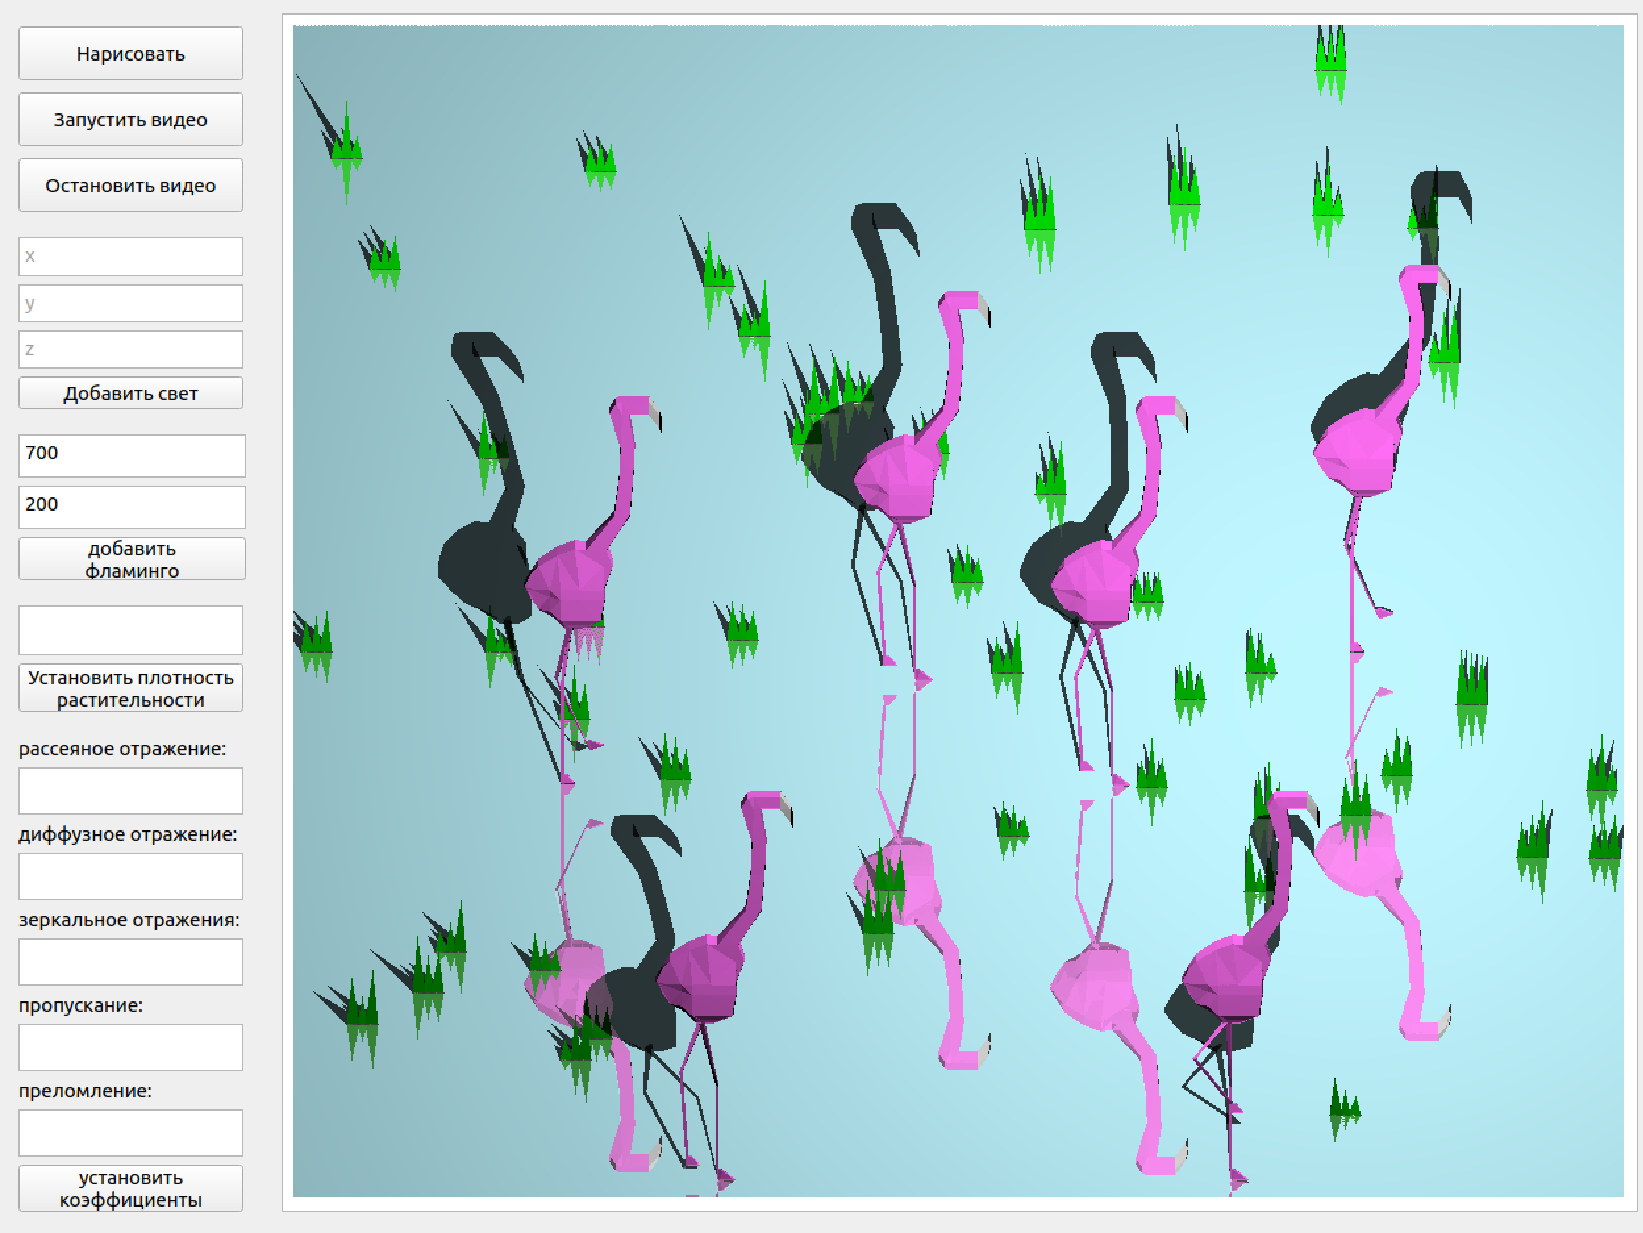
\includegraphics[width=0.9\linewidth]{img/ex4}
	\caption{Пример работы программы 4}
	\label{fig:ex4}
\end{figure}

\begin{figure}[h!]
	\centering
	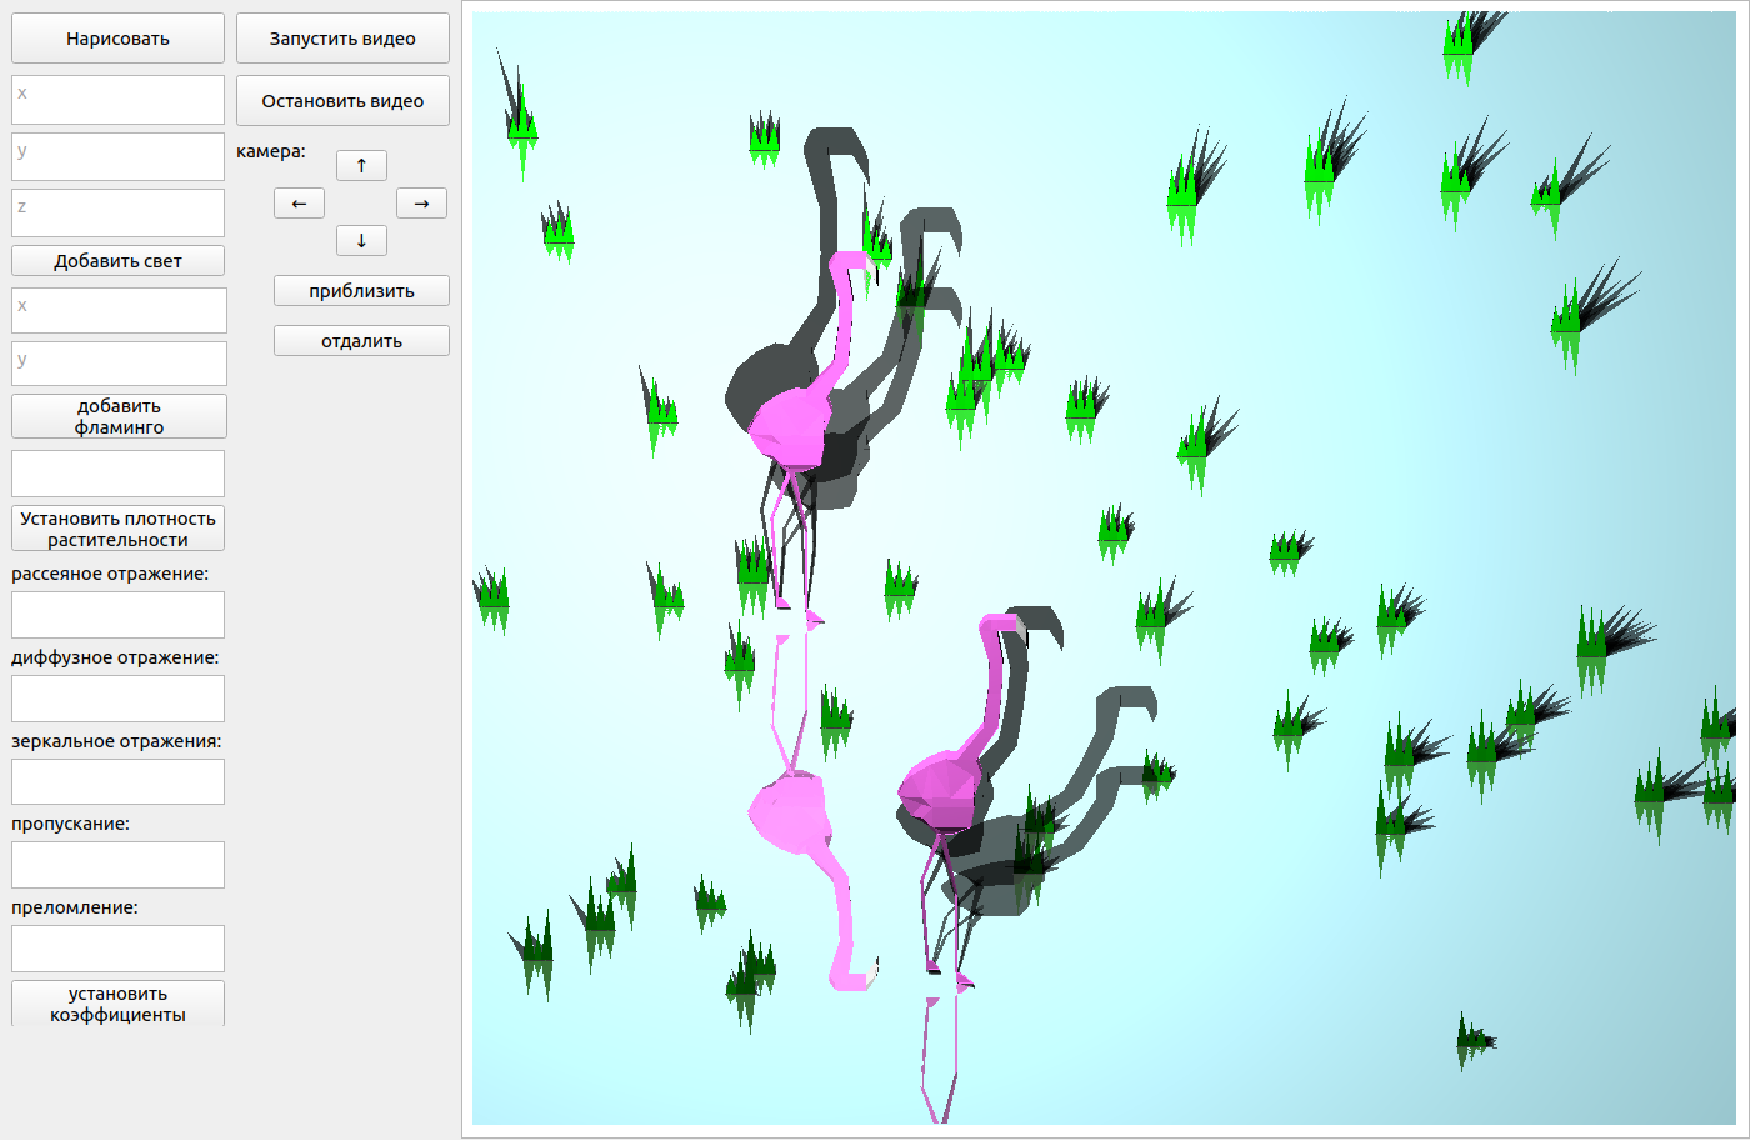
\includegraphics[width=0.9\linewidth]{img/ex5}
	\caption{Пример работы программы 5}
	\label{fig:ex5}
\end{figure}

\begin{figure}[h!]
	\centering
	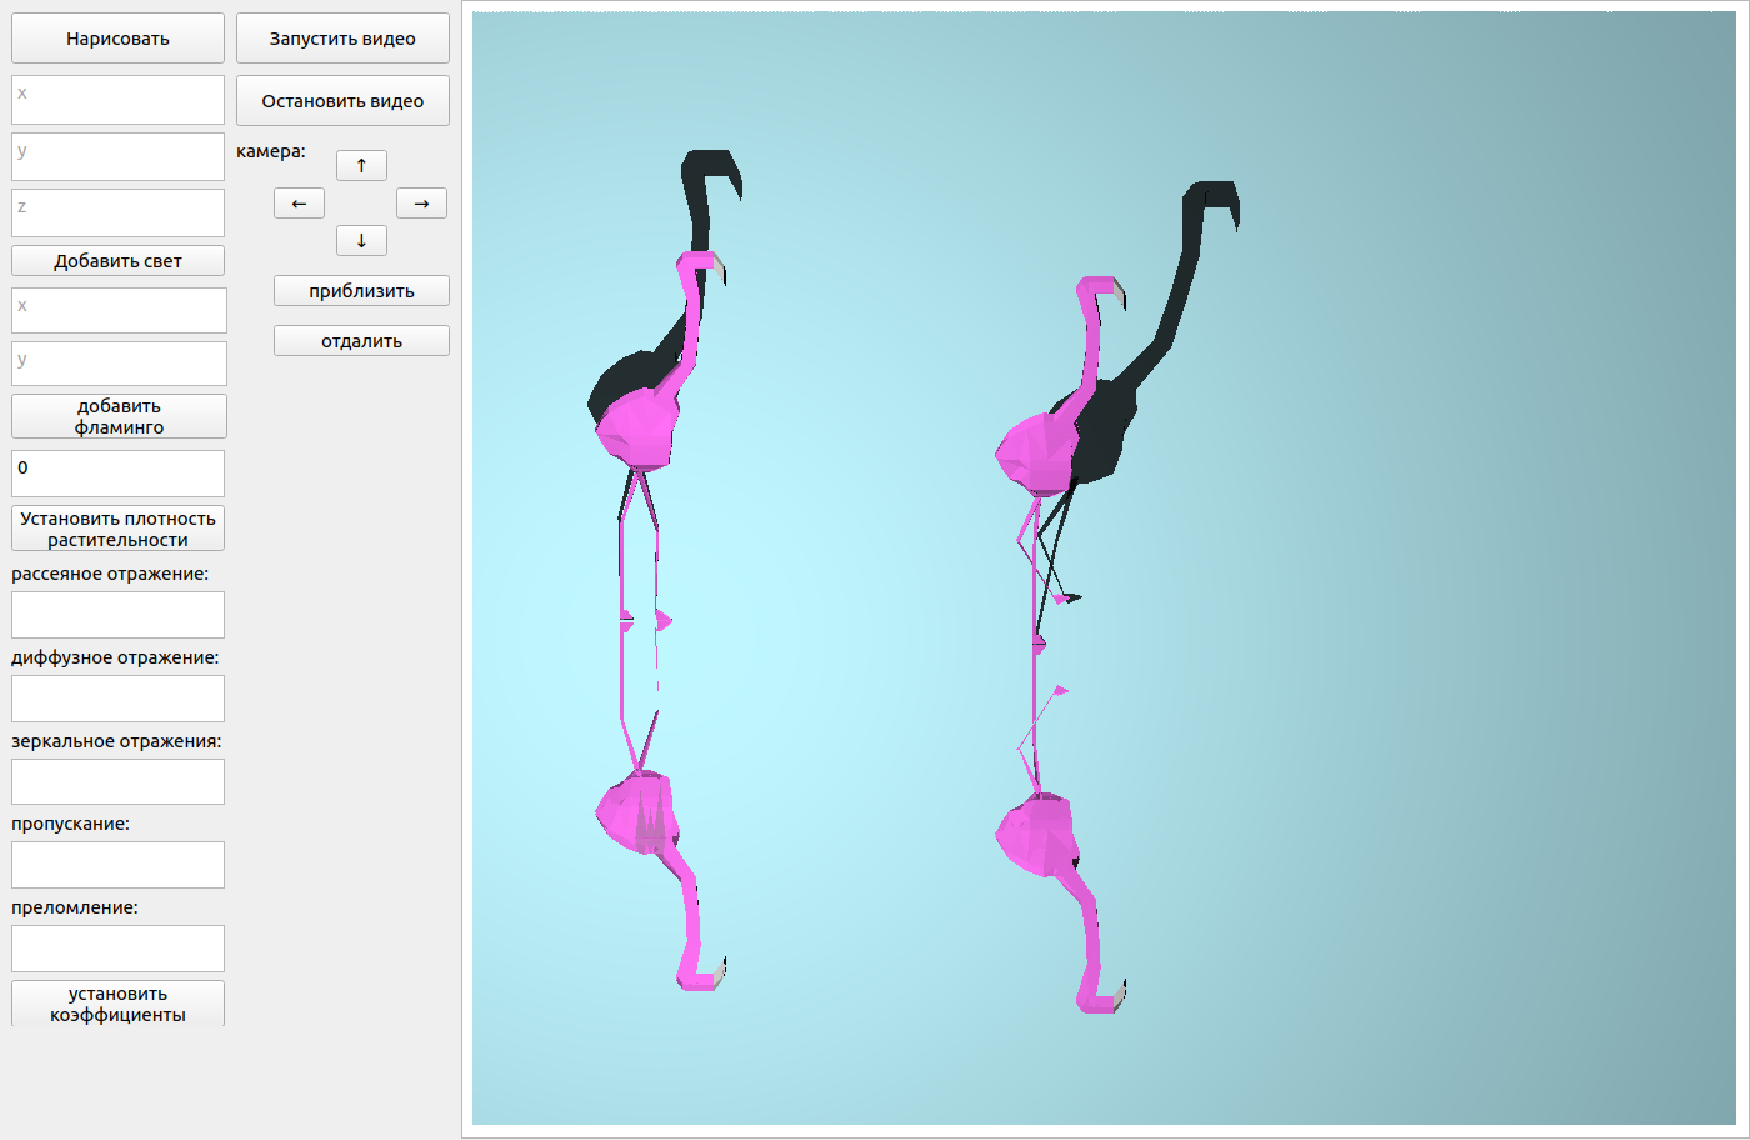
\includegraphics[width=0.9\linewidth]{img/ex7}
	\caption{Пример работы программы 6}
	\label{fig:ex6}
\end{figure}

\begin{figure}[h!]
	\centering
	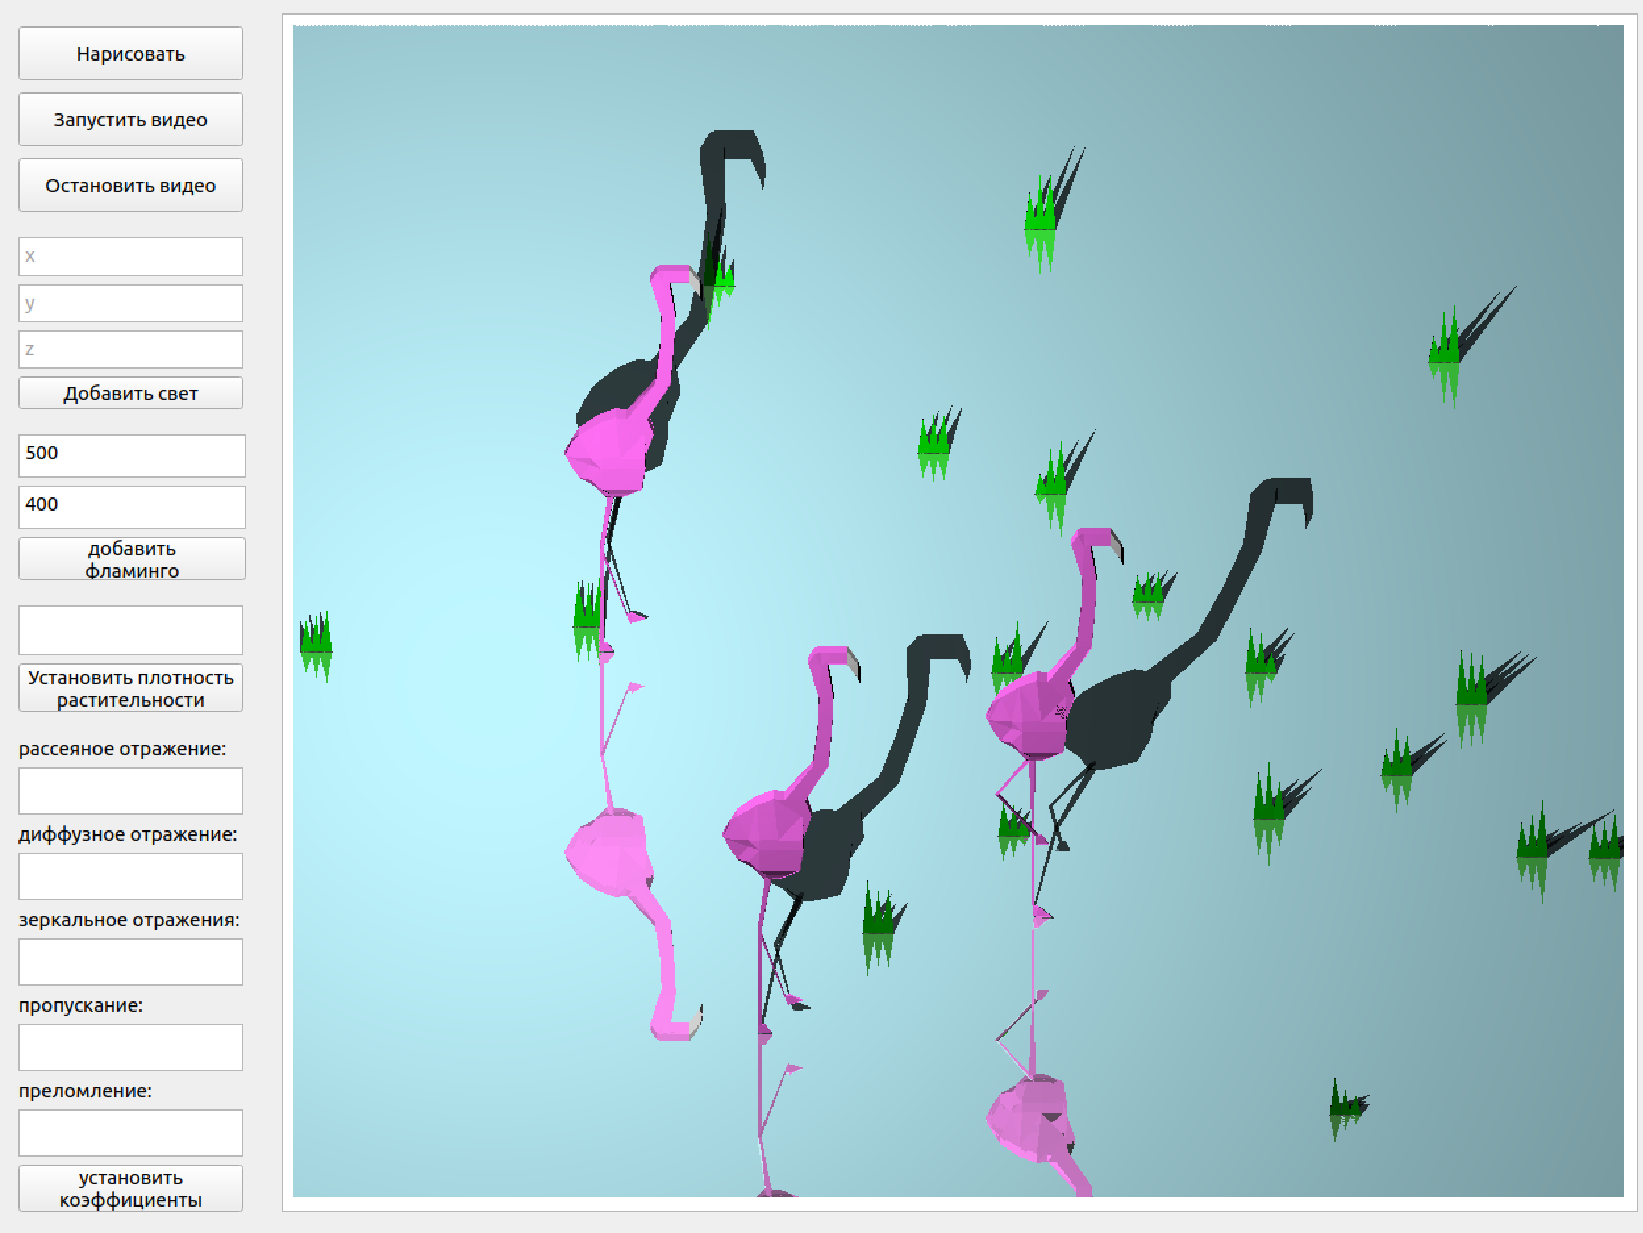
\includegraphics[width=0.9\linewidth]{img/ex6}
	\caption{Пример работы программы 7}
	\label{fig:ex7}
\end{figure}
\clearpage

\section{Функциональное тестирование}

Функциональным тестированием в данном случае является визуальное сравнение ожидаемого результата с полученным программой.
Функциональные тесты:
\begin{enumerate}[label=\arabic*)]
	\item на сцене отображается фламинго с растительностью на озере, что подтверждает рисунок~\ref{fig:ex1};
	\item на сцене могут отображаться одновременно несколько фламинго, что подтверждают рисунки~\ref{fig:ex2}--\ref{fig:ex4}.
	\item расположение источника света можно задать, что подтверждает рисунок~\ref{fig:ex5};
	\item можно задать несколько источников света, что подтверждает рисунок~\ref{fig:ex6};
	\item плотность растительности можно задать, что подтверждает рисунок~\ref{fig:ex7}. 
\end{enumerate}


\section*{Вывод}

В данной части были рассмотрены средства реализации, разработано программное обеспечение, рассмотрен интерфейс и сценарии тестирования.